\chapter{Für Nerds}
\label{ch:fuerNerds}
\textit{Die eigene Sammlung auf der eigenen Homepage veröffentlichen. Mit Hilfe von Plugins für OpenCms kein Problem für PUMA.}
\section{URL-Syntax\index{URL-Syntax}}
\label{sec:urlSyntax}
Sie können die Funktionen von PUMA nicht nur über das Menü (\autoref{sec:hauptmenue}) erreichen, sondern auch direkt über die URL ansteuern. Die URL ist die Adresse einer Seite, die im Adressfeld des Browsers eingegeben, bzw. angezeigt wird. Die Seite mit der Adresse \texttt{\begin{small}https://puma.ub.uni-stuttgart.de/user/mueller/forschungsdaten\end{small}} liefert beispielsweise alle Einträge des Benutzers \textit{mueller} zurück, die mit dem Tag \textit{forschungsdaten} gekennzeichnet sind.
Der Teil \texttt{https://puma.ub.uni-stuttgart.de} bezeichnet den Ort der PUMA-Installation, der Rest der URL steuert, welche Seiten oder Inhalte von PUMA zurückgegeben werden. 
 
\subsection{Allgemeine Seiten}
\label{subsec:allgemeineSeiten}
\begin{description}
    \item [/] Homepage von PUMA, zeigt die aktuellsten 50 öffentlichen Einträge.
    \item [/popular] Zeigt die 100 häufigsten Einträge der letzten 100.000 öffentlichen Einträge.
    \item [/IhrBenutzername]    Ihre persönliche Sammlung.
    \item [/help\_de]    Hilfeseite.
     \item [/myBibTeX]    Zeigt Ihre gesamte Sammlung im BibTex-Format.
    \item [/myRelations]    Zeigt Ihre Konzepte/Relationen.
    \item [/myDuplicates]    Zeigt die Duplikaten, die sich in Ihrer eigenen Sammlung befinden.
    \item [/groups]   Zeigt eine Liste aller Gruppen, die es in PUMA gibt.
    \item [/mySearch] Bietet eine Schnellsuche in Ihrer eigenen Sammlung.

\end{description}    

\subsection{Administrative Seiten}
\label{subsec:adminSeiten}
\begin{description}
\item [/settings]  Einstellungsseite. Auf dieser Seite können Sie:
    \begin{itemize}
        \item Ihr Profil bearbeiten und Kontoeinstellungen ändern,
        \item einen Benutzer zu Ihrer Gruppe hinzufügen,
        \item Ihren API-Schlüssel finden und einen neuen erzeugen,
        \item Ihr Passwort ändern und
        \item Ihre Daten zwischen BibSonomy und PUMA synchronisieren.
    \end{itemize}
    \item [/postBookmark]    Neues Lesezeichen einfügen. \hfill \\Überprüft vorab, ob sich die URL der Seite bereits in der Sammlung befindet.
    \item [/postPublication]    Neue Publikation einfügen. 
\end{description}

\subsection{Publikations- und Lesezeichenlisten nach verschiedenen Kriterien erstellen}
\label{subsec:suchenMitUrlSyntax}
PUMA bietet Ihnen die Möglichkeit mit Hilfe der URL ihre Publikationslisten nach verschiedenen Kriterien zusammenzustellen und zu filtern. Möglichke Kriterien sind: Tags, Autor, Publikationsjahr, Benutzername der Person, die den Eintrag gespeichert hat, sowie Freunde- und Gruppennamen. 

\subsubsection*{Einträge nach Benutzer}
\label{sss:nachBenutzer}

Um die Einträge eines bestimmten Benutzers aufzulisten, verwenden Sie die Syntax \texttt{/user/<benutzername>}, wobei \texttt{<benutzername>} für den PUMA-Benutzername des gewünschten Nutzers steht. Das Ergebnis kann zusätzlich noch nach Tag gefiltert werden: \texttt{/user/<benutzername>/<tag>}. Mehrere Tags können durch ein + verknüpft werden.

Beispiele:
\begin{description}
    \item [/user/eckert] \hfill \\ 
    Zeigt alle öffentlichen Einträge des Benutzers \textit{eckert}.
    \item [/user/eckert/politik] \hfill \\
    Zeigt alle öffentlichen Einträge mit dem Tag \textit{politik} des Benutzers \textit{eckert}.
    \item [/user/eckert/politik+menschenrechte] \hfill \\
    Zeigt alle öffentlichen Einträge des Benutzers \textit {eckert} an, die sowohl mit dem Tag \textit{politik} als auch mit dem Tag \textit{menschenrechte} annotiert sind.
\end{description}

\subsubsection*{Einträge nach Tag\index{Tags}}
\label{sss:nachTag}
Um alle Einträge aufzulisten, die mit einem bestimmten Tag annotiert sind, verwenden Sie die Syntax \texttt{/tag/<tag>}, wobei <tag> durch das gewünschte Tag ersetzt wird. Mehrere Tags können mit einem + verknüpft werden.

Beispiele:
\begin{description}
    \item [/tag/politik] \hfill \\
    Zeigt alle öffentlichen Einträge mit dem Tag \textit{politik} an.
    \item [/tag/politik+menschenrechte] \hfill \\
    Zeigt alle öffentlichen Einträge an, die sowohl mit dem Tag \textit{politik} als auch mit dem Tag \textit{menschenrechte} annotiert sind.
\end{description}

\subsubsection*{Einträge nach Autor\index{Autoren}}
\label{sss:nachAutor}

Um alle Publikationen eines bestimmten Autors aufzulisten, verwenden Sie die Syntax \texttt{/autor/<name>}, wobei <name> durch den Nachnamen des Autors ersetzt wird. Die Liste lässt sich mit Hilfe der Syntax \texttt{/author/<name>/<tag>} auf bestimmte Tags eingrenzen oder durch \texttt{/author/<name>/sys:<systemtag>:<wert>} mit verschiedenen Systemtags (siehe auch \autoref{sss:systemtags}) weiter einschränken.

Beispiele:
\begin{description}
    \item [/author/müller] \hfill \\
    Zeigt alle Publikationen des Autors mit dem Namen \textit{Müller} an.
    \item [/author/müller/dblp] \hfill \\
    Zeigt alle Einträge des Autors \textit{Müller} an, die mit dem Tag \textit{dblp} annotiert sind
    \item [/author/müller/sys:user:eckert] \hfill \\
    Zeigt alle Publikationen des Autors \textit{Müller} in der Sammlung von \textit{Eckert} an.
    \item [/author/müller/sys:group:puma] \hfill \\
    Zeigt alle Publikationen des Autors \textit{Müller} in der Sammlung aller Gruppenmitglieder der Gruppe \textit{puma} an. 
\end{description}

Mit dem Systemtag \textit{year} lässt sich das Ergebnis auf ein bestimmtes Erscheinungsjahr oder einen bestimmten Zeitraum beschränken:%muss rausrücken

Beispiele:
\begin{description}
    \item [/author/hotho/sys:year:2007] \hfill \\
    Zeigt alle Publikationen des Autors \textit{Hotho} aus dem Jahre 2007.
    \item [/author/hotho/sys:year:2003-2007] \hfill \\
    Zeigt alle Publikationen des Autors \textit{Hotho} zwischen 2003 und 2007.
    \item [/author/hotho/sys:year:-2005] \hfill \\
    Zeigt alle Publikationen des Autors \textit{Hotho} bis zum Jahr 2005 an.
    \item [/author/hotho+sys:year:1997-] \hfill \\
    Zeigt alle Publikationen des Autors \textit{Hotho} seit 1997 an.
\end{description}

\subsubsection*{Einträge von Freunden} 
\label{sss:vonFreunden}
Um die Einträge Ihrer Freunde (\autoref{sec:freunde}) zu sehen, verwenden Sie die Syntax \texttt{/friends} für alle Freunde oder \texttt{/friend/<name>} für die Einträge eines bestimmten Freundes. Sie können die Ergebnisse wie gewohnt durch die Angabe von Tags weiter einschränken. 

Sie sehen nur die Einträge, die von Benutzern stammen, auf deren Freundesliste Sie stehen und die von diesen Benutzern für Freunde freigegeben wurden (für Freunde sichtbar).

Beispiele:
\begin{description}
    \item [/friends] \hfill \\
    Zeigt die für Freunde sichtbaren Einträge aller ihrer Freunde.
    \item [/friend/eckert] \hfill \\
    Zeigt die für Freunde sichtbaren Einträge des Benutzers \textit{eckert}. Sie können diese Einträge nur dann sehen, wenn \textit{eckert} Sie als Freund angegeben hat.
    \item [/friend/eckert/politik] \hfill \\
    Zeit die für Freunde sichtbaren Einträge des Benutzers \textit{eckert} an, die mit dem Tag \textit{politik} annotiert wurden. 
    \item [/friend/eckert/politik+menschenrechte] \hfill \\
    Zeigt die für Freunde sichtbaren Einträge des Benutzers \textit{eckert} an, die sowohl mit dem Tag \textit{politik} als auch mit dem Tag \textit{menschenrechte} annotiert sind. 
\end{description}

\subsubsection*{Einträge nach Sichtbarkeit}
\label{sss:nachSichtbarkeit}
Um zu sehen, welche ihrer Einträge für wen sichtbar sind, können Sie die Syntax \texttt{/viewable/<sichtbarkeit>} verwenden. Als \texttt{<sichtbarkeit>} sind folgende Ausprägungen möglich:
\begin{description}
  \item[public] Einträge, die öffentlich sichtbar sind
	\item[private] Einträge, die nur für Sie selber sichtbar sind
	\item[friends] Einträge, die für die Benutzer sichtbar sind, die auf ihrer Freundeliste stehen
	\item[<gruppenname>] Einträge, die für die Mitglieder der Gruppe <gruppenname> sichtbar sind
\end{description}  

Die Ergebnisse können mit Hilfe der Syntax \texttt{/viewable/<sichtbarkeit>/<tags>} zusätzlich durch Tags eingeschränkt werden. 

Beispiele:
\begin{description}
    \item [/viewable/public] \hfill \\
    Zeigt alle Ihre Einträge an, die Sie als \enquote{öffentlich sichtbar\index{Sichtbarkeit!öffentlich}} eingestellt haben.
    \item [/viewable/public/politik] \hfill \\
    Zeigt alle Ihre öffentlich sichtbaren Einträge, die mit dem Tag \textit{politik} annotiert wurden.
    \item [/viewable/private] \hfill \\
    Zeigt alle Ihre Einträge, die Sie als \enquote{privat sichtbar\index{Sichtbarkeit!privat}} eingestellt haben.
    \item [/viewable/private/politik+menschenrechte] \hfill \\
    Zeigt alle Ihre Einträge an, die nur für Sie sichtbar sind und sowohl mit dem Tag \textit{politik} als auch mit dem Tag \textit{menschenrechte} annotiert wurden. 
    \item [/viewable/friends] \hfill \\
    Zeigt alle Ihre Einträge an, die Sie als \enquote{für Freunde sichtbar\index{Sichtbarkeit!Freunde}} eingestellt haben.
    \item [/viewable/puma] \hfill \\
    Zeigt alle Einträge an, die für die Gruppe \textit{puma} als sichtbar eingestellt wurden.
    \item [/viewable/puma/politik] \hfill \\
    Zeigt alle Einträge an, die für die Gruppe \textit{puma} sichtbar sind und mit dem Tag \textit{politik} annotiert wurden.
\end{description}

\subsubsection*{Einträge nach Gruppe\index{Gruppen}}
\label{sss:nachGruppe}
Wenn Sie Mitglied einer Gruppe (\autoref{sec:gruppen}) sind, können Sie mit Hilfe der Syntax \texttt{/group/<gruppenname>} die Einträge aller Gruppenmitglieder auflisten. Die Ergebnisse können mit \texttt{/group/<gruppenname>/<tags>} nach Tags gefiltert werden.

Beispiele:
\begin{description}
    \item [/group/puma] \hfill \\
    Zeigt Ihnen alle Einträge von Mitgliedern der Gruppe \textit{puma} an, wenn Sie selber Gruppenmitglied sind.
    \item [/group/puma/politik] \hfill \\
    Zeigt Ihnen alle Einträge von Mitgliedern der Gruppe \textit{puma} an, die mit dem Tag \textit{politik} annotiert sind. 
    \item [/group/puma/politik+menschenrechte] \hfill \\
    Zeigt Ihnen alle Einträge von Mitgliedern der Gruppe \textit{puma} an, die mit dem Tag \textit{politik} und dem Tag \textit{menschenrechte} annotiert sind. 
    \item [/relevantfor/group/puma] \hfill \\
    Zeigt Ihnen alle Einträge an, die ein Gruppenmitglied der Gruppe \textit{puma} als relevant für diese Gruppe gekennzeichnet hat.
    \item [/followers] \hfill \\
    Zeigt die neuesten Einträge aller Benutzer, denen Sie folgen. Diese Einträge werden mittels eines Rankings so umsortiert, dass die für Sie relevantesten Einträge ganz oben stehen. 
\end{description}



\paragraph*{Umgang mit Duplikaten\index{Duplikate}}
\label{subsec:duplikate}
Wenn innerhalb einer Gruppe zwei oder mehr Benutzer denselben Eintrag in ihrer Sammlung haben, kommt es vor, dass Einträge (Publikationen) mehrfach auf einer Gruppenseite angezeigt werden. Falls dies nicht gewünscht ist, kann das Verhalten mittels des Parameters \textit{duplicates} angepasst werden. Der Parameter kann folgende Ausprägungen haben:
\begin{description}
\item [yes] Jeder Eintrag wird angezeigt, auch wenn er ein Duplikat darstellt (Standard).
  \item[no] Bei Duplikaten wird jeweils nur der erste Eintrag angezeigt.
  \item [merged] Die Tags aller Duplikate werden gesammelt an einem einzelnen Eintrag angezeigt.
  \end{description}

Beispiele:
\begin{description}
    \item [/group/puma?duplicates=no] \hfill \\
    Zeigt alle Einträge der Gruppe \textit{puma} an. Für jedes Duplikat wird nur der erste Eintrag angezeigt.
    \item [/group/puma?duplicates=merged] \hfill \\
    Zeigt alle Einträge der Gruppe \textit{puma} an. Für jedes Duplikat werden alle Tags \enquote{aufgesammelt} und aggregiert an einem einzelnen Eintrag angezeigt.
\end{description}

Weitere Parameter finden Sie im \autoref{subsec:parameter}.

\subsubsection*{Weitere Filterkriterien}
\label{sss:weitereKriterien}

PUMA bietet noch weitere Kriterien, nach denen Ergebnislisten zusammengestellt und gefiltert werden können. Mit der Syntax \texttt{/url/<hashkey>} werden alle Lesezeichen angezeigt, deren URL den Hash <hashkey> haben. Veröffentlichnungen mit einem bestimmten Intra-Hash (siehe \autoref{sec:duplikat}) erreichen Sie mit der Syntax \texttt{/bibtex/<intrahash>}. Mit der Syntax \texttt{/bibtexkey/<bibtexkey>} können Sie Veröffentlichungen mit einem bestimmten BibTeX-Key anzeigen.


\subsection{Konzeptseiten}
\label{subsec:konzeptseiten}
Konzepte (\autoref{subsec:konzepte}) sind Überbegriffe, mit denen Sie Ihre Tags strukturiert können. Um die Konzepte eines Benutzers anzuzeigen, verwenden Sie die Syntax \texttt{/concepts/<benutzername>}. Um die Lesezeichen oder Publikationen zu erhalten, die mit einem Konzept oder eines seiner Untertags annotiert wurden, verwenden Sie die Syntax \texttt{/concept/user/<benutzername>/<konzept>}.

Beispiele:
\begin{description}
    \item [/concepts/eckert] \hfill \\
    Zeigt alle Konzepte\index{Konzepte} des Benutzers \textit{eckert}.
    \item [/concept/user/eckert/psychologie] \hfill \\
    Zeigt alle Lesezeichen und Publikationen des Benutzers \textit{eckert} an, denen das Konzept \textit{psychologie} oder eines seiner Unterschlagwörter als Tag zugeordnet ist. 
\end{description}

\subsection{Volltextsuche}
\label{subsec:volltext}
Die Volltextsuche von PUMA wird über die URL-Syntax \texttt{/search/<suchbegriff>} gesteuert. Mehrere Suchbegriffe können mit einem \texttt{+} verknüpft werden. Ein \texttt{-} vor einem Suchbegriff bewirkt, dass nur Einträge zurückgeliefert werden, die den entsprechenden Suchbegriff \textbf{nicht} enthalten. Ein Suchbegriff kann mit der Syntax \texttt{user:<benutzername>} auch den Benutzer festlegen, in dessen Einträgen gesucht werden soll.

Die Volltextsuche sucht in den Feldern Titel und Beschreibung (bei Lesezeichen auch noch in der URL) nach allen Einträgen, die den Suchbegriff oder die Suchbegriffe enthalten.

Beispiele:
\label{subsec:volltextsuche}
\begin{description}
    \item [/search/politik] \hfill \\
    Zeigt alle öffentlichen Einträge an, die das Wort \textit{politik} enthalten. 
    \item [/search/politik+menschenrechte] \hfill \\
    Zeigt alle öffentlichen Einträge, die das Wort \textit{politik} und das Wort \textit{menschenrechte} enthalten. 
    \item [/search/politik+-menschenrechte] \hfill \\
    Zeigt alle öffentlichen Einträge, die das Wort \textit{politik}, aber nicht das Wort \textit{menschenrechte} enthalten. 
    \item [/search/politik+user:droessler] \hfill \\
    Zeigt alle öffentlichen Einträge des Benutzers \textit{droessler}, die das Wort \textit{politik} enthalten. 
    \item [/search/politik+menschenrechte+user:droessler] \hfill \\
    Zeigt alle öffentlichen Einträge des Benutzers \textit{droessler} an, die das Wort \textit{politik} und das Wort \textit{menschenrechte} enthalten. 
    \item [/search/politik+-menschenrechte+user:droessler] \hfill \\
    Zeigt alle öffentlichen Einträge des Benutzers \textit{droessler} an, die das Wort \textit{politik}, aber nicht das Wort \textit{menschnerechte} enthalten. 
\end{description}


\subsection{Export von Einträgen}
\label{subsec:export}
PUMA bietet Ihnen die Möglichkeit, Ihre Lesezeichen und Publikationen in viele verschiedene Formate zu exportieren.
Die Exportfunktion von PUMA steuern Sie mit der Syntax \texttt{/<exportformat>}. Als Exportformat können Sie aus den folgenden Möglichkeiten wählen.

\begin{itemize}
    \item RSS Feeds\index{RSS}
    \begin{description}
        \item [/publrss/] Liefert einen RSS-Feed zurück.
        \item [/burst/]  Liefert einen BuRST-Feed zurück.
        \item [/aparss/] Liefert einen RSS-Feed im APA-Format zurück.
    \end{description}
    \item Strukturierte Daten
    \begin{description}
        \item [/bib/] Gibt die Einträge im BibTeX-Format\index{BibTex} zurück.
        \item [/endnote/] Gibt die Einträge im EndNote-Format\index{EndNote} zurück.
        \item[/json/] Gibt die Einträge im JSON-Format zurück.
        \item[/swrc/] Gibt die Einträge im  RDF-Format gemäß der SWRC-Ontologie für das Semantic Web zurück.
    \end{description}
    \item HTML\index{HTML}
    \begin{description}
        \item [/publ/] Gibt die Einträge als HTML-Tabelle zurück.
        \item [/publ/?notags=1] Gibt die Einträge ohne Tags als HTML-Tabelle zurück.
    \end{description}
  \item JabRef-Layouts
    \begin{description}
  \item[/layout/simplehtml/] Gibt die Einträge im HTML-Format als einfache Auflistung zurück.
  \item[/layout/html/] Gibt die Einträge im HTML-Format als formatierte Aufzählung zurück.
  \item[/layout/tablerefs/] Gibt die Einträge im HTML-Format als durchsuchbare Tabelle zurück.
  \item[/layout/tablerefsabsbib/] Gibt die Einträge im HTML-Format als durchsuchbare Tabelle zusätzlich mit aufklappbarem Abstract und BibTeX-Eintrag zurück.
  \item[/layout/docbook/] Gibt eine XML-Datei im Docbook-Format zurück.
  \item[/layout/dblp/] Gibt eine XML-Datei im DBLP-Format zurück.
  \item[/layout/endnote/] Gibt eine Text-Datei zurück, die vom Literaturverwaltungsprogramm EndNote verarbeitet werden kann
  \item[/layout/text/] Gibt eine Text-Datei im BibTeX-Format zurück.
    \end{description}
\end{itemize}

Die zu exportierenden Einträge können Sie dann über die Syntax \texttt{/<exportformat>/user/<benutzername>/<tags>} nach Benutzer filtern und auch zusätzlich noch auf bestimmte Tags einschränken. Möchten Sie nur nach Tag und nicht nach Benutzer filtern, verwenden Sie die Syntax \texttt{/<exportformat>/tag/<tags>}. Analog können Sie auch die anderen Kriterien zur Filterung der Ausgabe verwenden, die im \autoref{subsec:suchenMitUrlSyntax} beschrieben sind.

Beispiele:
\label{subsec:volltextsuche}
\begin{description}
    \item [/bib/user/droessler] \hfill \\
    Gibt alle Einträge des Benutzers \textit{droessler} im BibTeX-Format aus.
    \item [/publrss/group/testgroup] \hfill \\
      Liedert einen RSS-Feed zurück, der die Einträge der Gruppe \textit{testgroup} enthält.
    \item [/layout/tablerefs/tag/fdm] \hfill \\
      Gibt eine durchsuchbare Tabelle im HTML-Format zurück, die alle Einträge mit dem Tag \textit{fdm} enthält. 
\end{description}

%nach hinten verschieben
\subsection{Parameter}
\label{subsec:parameter}
Mit einem Fragezeichen können an eine URL Parameter angehängt werden, die die Ausgabe steuern (Sortierung, Anzahl angezeigter Einträge).

Mehrere Parameter werden durch ein \& getrennt. Die URL \texttt{\begin{small} /user/mueller?items=25\&sortPage=author\&sortPageOrder=desc\end{small}} liefert zum Beispiel die ersten 25 Einträge des Benutzers \textit{mueller} absteigend sortiert nach Autor. 

Immer wenn Sie in PUMA eine Liste von Lesezeichen oder Publikationen ausgeben, können Sie diese sortieren, indem Sie an die URL einen oder mehrere der folgenden Suchparameter anhängen. Folgende Parameter stehen Ihnen zur Verfügung:
\begin{description}
    \item [sortPage] Wonach wird sortiert?
    \begin{description}
        \item [author] Autorenname
        \item [editor] Herausgebername
        \item [year] Erscheinungsjahr
        \item [entrytype] Publikationstyp
        \item [title] Titel
        \item [booktitle] Buchtitel (insb. bei Artikel in Sammelbänden)
        \item [journal] Journalname
        \item [school] Universitätsname 
    \end{description}
    \item [sortPageOrder] Reihenfolge der Sortierung
    \begin{description}
        \item [asc] aufsteigend
        \item [desc] absteigend 
    \end{description}
\end{description}

Die Parameter \texttt{items} und \texttt{duplicates} steuern wieviele Einträge mit oder ohne Duplikate angezeigt werden:

\begin{description}		
    \item [items] Wieviele Einträge werden angezeigt\hfill \\
		 Wenn dieser Parameter nicht angegeben ist, werden standardmäßig 20 Einträge angezeigt.
    \item [duplicates] Duplikate\index{Duplikate}
    \begin{description}
        \item [yes] Erlaubt Duplikate in der Lesezeichen/- Publikationsliste
        \item [no] Entfernt Duplikate aus der Ergebnisliste
    \end{description}
\end{description}
%Beispiel: \url{?sortPage=year%\&sortPageOrder=asc\&duplicates=no} \newline
%Beispielkasten einfuegen
%Sortiere nach Erscheinungsjahr (sortPage=~year) aufsteigend (sortPageOrder=~asc) und entferne alle Duplikate (duplicates=~no). \newline


\section{Duplikatserkennung\index{Duplikat}} 
\label{sec:duplikat}
Die Duplikatserkennung von PUMA basiert auf Hashkeys. PUMA berechnet für jede Publikation zwei Hash Keys, den intrahash (zur Duplikatserkennung innerhalb der Sammlung eines Benutzers) und den interhash (zur Duplikatserkannung zwischen den Sammlungen verschiedener Benutzer). Zur Berechnung der Keys werden Titel, Autor und Jahr (beim intrahash zusätzlich noch Typ, Zeitschriften- oder Buchtitel, Band und Nummer) aneinander gefügt und ein Hash-Wert über dieser Zeichenfolge berechnet. Wird nun eine Publikation zum zweiten Mal in die Sammlung eingetragen, vergibt PUMA an diese Publikation den gleichen, schon vorhandenen Hashkey. Das System bemerkt die doppelte Vergabe und kennzeichnet die Publikationseinträge als Duplikate. 


\section{REST-API\index{REST-API}}
\label{sec:restApi}
PUMA bietet einen Webservice auf REST-Basis (Representational State Transfer) an. REST-Schnittstellen basieren auf dem HTTP-Protokoll und bedienen sich der Befehle GET (Informationen abrufen), POST (neue Einträge anlegen), PUT (bestehende Einträge aktualisieren) und DELETE (Einträge löschen). Die REST-Schnittstelle von PUMA dient dazu, anderen Programmen oder Skripten Zugriff auf die Daten und Funktionalitäten von PUMA zu geben. Damit wird eine automatisierte Verarbeitung der in PUMA gespeicherten Sammlungen möglich.

\subsection{API-Clients für verschiedene Programmiersprachen}
\label{subsec:apiClients}
Um die Ansprache der API zu erleichtert, gibt es für verschiedene Programmiersprachen Pakete oder Bibliotheken, die bereits einen Client implementiert haben, der die Kommunikation mit der REST-API übernimmt.

\begin{description}
\item [Java] \hfill \\
  Der bibsonomy-rest-client \footnote{\url{https://bitbucket.org/bibsonomy/bibsonomy/src/tip/bibsonomy-rest-client/}} ist ein Java-Modul, das die Kommunikation mit der REST-API von PUMA erleichtert. Zur API gibt es eine ausführliche Dokumentation mit Beispielen\footnote{\url{https://bitbucket.org/bibsonomy/bibsonomy/wiki/documentation/api/Java\%20API\%20Examples}}. Als PUMA-Nutzer muss die URL (endpoint) auf \textit{https://puma.ub.uni-stuttgart.de/} gesetzt werden.
\item [PHP] \hfill \\
  Die restclientp-php Bibliothek\footnote{\url{https://bitbucket.org/bibsonomy/restclient-php/}} bietet einen API-Client für PUMA und Bibsonomy. Als \texttt{\$baseurl} verwenden Sie \textit{https://puma.ub.uni-stuttgart.de}.
\item [Python] \hfill \\
 Für Python gibt es eine Bibsonomy-Klasse\footnote{\url{https://bitbucket.org/bibsonomy/bibsonomy-python/}}, die die Anfragen auf die REST-Schnittstelle implementiert. Als PUMA-Nutzer geben Sie bei der Initialisierung neben ihrem Benutzernamen als \texttt{user\_name} und ihrem API-Key als \texttt{api\_key} auch noch \textit{puma.ub.uni-stuttgart.de} als \texttt{hostname} an.

\end{description}

\subsection{Authentifizierung zum Zugriff auf die API}
\label{subsec:apiAuth}\label{sss:apiKey}

Um per API-Schnittstelle auf Ihre Inhalte in PUMA zugreifen zu können, müssen Sie sich  mit einem individuellen API-Key gegenüber PUMA authentifizieren. Eine Authentifizierung über OAuth wird nicht unterstützt.

Ihren individuellen API-Key finden Sie in den Einstellungen (\autoref{sec:einstellungen}) im Reiter \textit{Einstellungen} unter \textit{API}. An dieser Stelle haben Sie auch die Möglichkeit, einen neuen Key zu erzeugen. 

\section{Integration von PUMA-Inhalten auf eigenen Webseiten}
\label{sec:eigeneWebseiten}
Es gibt mehrere Möglichkeiten, Inhalte aus PUMA oder Links zu PUMA auf Ihrer eigenen Webseite zu integrieren.

\subsection{Bookmarklinks\index{Bookmarklinks}}
\label{subsec:bookmarklinks}
Mit Hilfe eines kurzen JavaScript\index{JavaScript}-Codes\footnote{zu finden unter \url{https://ub.uni-stuttgart.de/buttons}} können Sie einen Link auf Ihrer Seite einfügen, mit dem die Besucher Ihre Seite mit einem Klick in ihre eigene PUMA-Sammlung übernehmen können.
\lstset{language=JavaScript}
\begin{lstlisting}
  <!-- post bookmark link code -->
  <script type="text/javascript">
    var url = encodeURIComponent(document.location.href);
    var title = encodeURIComponent(document.title);
    var pumaUrl = "https://puma.ub.uni-stuttgart.de"
       + "/ShowBookmarkEntry?"
       + "url=" + url
       + "&description=" + title;
    var linkCode = "<a href=\"" + pumaUrl + "\""
    + " rel=\"nofollow\""
    + " title=\"Bookmark this page to PUMA.\">"
    + "Bookmark to PUMA!</a>"
    document.write(linkCode);
  </script>
\end{lstlisting}

\subsection{iFrame}
\label{subsec:iFrame}
Mit Hilfe eines iFrames können Sie beliebige PUMA-Seiten im PUMA-Layout auf Ihrer Seite integrieren. 
\lstset{language=HTML}
\begin{lstlisting}
  <iframe
  src="<UrlPumaSeite>?format=embed">

  </iframe>''
\end{lstlisting}

Sie können als \texttt{src} jede beliebige PUMA-Seite verwenden. Möchten Sie zum Beispiel eine Liste ihrer eigenen Publikationen \index{Publikationslisten!Eigene Publikationslisten} auf Ihrer Webseite einfügen, ersetzen Sie <UrlPumaSeite> durch \begin{small}https://puma.ub.uni-stuttgart.de/user/<benutzername>/myown\end{small}, wobei Sie für <benutzername> Ihren PUMA-Benutzernamen einsetzen.

Der Parameter \texttt{format=embed} sorgt dafür, dass nur die Inhalte und nicht die ganze PUMA-Seite integriert wird. Weitere Parameter finden Sie unter \autoref{subsec:parameter}.

\subsection{JSON-Feed\index{JSON-Feed}}
\label{subsec:jsonFeed}
Sie können für jede PUMA-Seite einen JSON-Feed\footnote{\url{http://www.json.org/}} generieren, indem Sie \textit{json/} vor den Pfadteil der URL stellen. Um beispielsweise einen JSON-Feed mit allen Einträgen zu bekommen, die mit dem Tag \textit{fdm} annotiert wurden, geben Sie \textit{/json/tag/fdm} ein (siehe auch \autoref{subsec:export}). 

Um die Inhalte des  JSON-Feeds auf Ihrer Seite anzuzeigen, können Sie beispielsweise die JavaScript-Bibliothek Exhibit \footnote{\url{http://www.simile-widgets.org/exhibit/}} verwenden. Der folgende Code stellt eine Publikationsliste aus PUMA als JSON-Feed für Exhibit zur Verfügung.

\lstset{language=HTML}
\begin{lstlisting}
  <link
    href="https://puma.ub.uni-stuttgart.de/json/tag/fdm"
    type="application/jsonp"
    rel="exhibit/data"/> 
\end{lstlisting}

Exhibit bietet dann eine Reihe von Möglichkeiten, die Daten zu filtern, zu sortieren und in verschiedenen Formaten auszugeben.

\section{Plugins} 
\label{sec:plugins}
\subsection{OpenCms\index{OpenCms}}
\label{subsec:opencms}
Mit dem OpenCms\index{Plugins!OpenCms} Plugin lassen sich Publikationslisten aus PUMA in OpenCms integrieren. Ein typischer Anwendungsfall des Plugins ist das Erstellen einer Instituts\-publi\-kations\-liste: Mitarbeiter und/~oder Hilfskräfte des Instituts pflegen die Publikationsdaten in PUMA ein. Die eingetragenen Publikationen können in einer Instituts\-publi\-kations\-liste ausgegeben und auf der Instituts\-website veröffentlicht werden. Hierbei kann zwischen mehreren Zitationsstilen ausgewählt und nach Datum in absteigender oder aufsteigender Reihenfolge sortiert werden. Das Gleiche können die Mitarbeiter ebenfalls für ihre eigenen Publikationslisten machen.
\subsubsection*{Umsetzung:}\label{sss:iplPuma}
\begin{enumerate}
\item  Anmeldung auf \url{https://puma.ub.uni-stuttgart.de.}
\item Legen Sie eine Gruppe an.
\item Mitarbeiter und/oder Hilfskräfte des Instituts tragen die
  Publikationen mit ihrem PUMA-Konto ein und annotieren diese mit dem
  Systemtag \textit{for:<gruppenname>}, wobei Sie <gruppenname>
  ersetzen durch den Namen der angelegten Gruppe.
\item Platzieren Sie auf einer Freitextseite in OpenCms den Typ \enquote{Publikationsliste aus BibSonomy/~PUMA} aus dem Typenkatalog.
\item Füllen Sie die Eingabefelder aus.
\end{enumerate}
%\newline\newline
Eine kurze Beschreibung der Eingabefelder:\newline
%\small
\begin{longtabu}{|X|p{7cm}|}\hline
\bfseries Eingabefeld &\bfseries Beschreibung\\ \hline
Titel& 	Der Titel ist frei wählbar und erscheint auf der Seite als Überschrift, z. B. Meine Publikationen. \\ \hline
API-Benutzer­­name &	Der API-Benutzername entspricht dem von Ihnen genutzten Benutzernamen bei PUMA. Er beginnt nach dem @-Zeichen und erscheint nach dem Login oben rechts im Benutzermenü.\\ \hline
API-Schlüssel &	Der API-Schlüs­sel ist ein Zahlencode, den Sie in Ihrem Benutzermenü (\autoref{sec:benutzermenue}) unter \enquote{Einstellungen} im Reiter \enquote{Einstellungen} finden und kopieren können.\\ \hline
API-Server &	Der API-Server ist bereits voreingestellt auf \url{https://puma.ub.uni-stuttgart.de/api/}\\ \hline
Quelle & Es kann aus drei möglichen Quellen ausgewählt werden: \textit{user} (Benutzerkonto), \textit{group} (Gruppenkonto) und \textit{viewable} (öffentliche Einträge im System). Für eine Institutspublikationsliste wird her \textit{group} eingetragen, für eine persönliche Publikationsliste \textit{user}.\\ \hline
Source-ID &	Im Feld Source-ID wird je nach gewählter Quelle der Benutzer- oder Gruppenname eingetragen. Für eine Institutspublikationsliste wird hier der Name der in Punkt 2 angelegten Gruppe eingetragen, für eine persönliche Publikationsliste der Benutzername. 
\\ \hline
Tags &	Mit diesem Feld kann die Liste auf die Einträge eingegrenzt werden, die mit dem oder den angegebenen Tag/s ausgezeichnet sind. Um eine Liste mit den eigenen Publikationen zu erstellen, wird hier \textit{myown} angegeben.\\ \hline
Exclude-Tags& An dieser Stelle werden die Schlagwörter angegeben, die in der Liste nicht vorkommen sollen.\\ \hline
Search &	Im Feld Search kann ein Suchbegriff eingegeben werden, nach dem die Ergebnisse per Volltextsuche durchsucht werden sollen. Sucht auch in hochgeladenen Volltexten.\\ \hline
Anzahl der Publikationen &	Gibt die Länge der Liste an. Standardwert 100 Einträge, Maximum 1000. \\ \hline
Sortierfeld &	Als Sortierfeld kann \textit{none} (keine Sortierung), \textit{author} (der Autor), \textit{entrytype} (der Publikationstyp), \textit{title} (der Titel) oder \textit{year} (das Jahr) gewählt werden.\\ \hline
Sortierreihenfolge &	Definiert, ob aufsteigend (ascending)- oder absteigend (descending) sortiert werden soll.\\ \hline 
Gruppierung &	Wenn angeklickt, wird die Ausgabe nach dem im Feld \textit{Sortierfeld} angegebenen Feld gruppiert. Bei \textit{author} und \textit{title} wird nach dem Alphabet (A,B,C, usw.) gegliedert. Bei \textit{entrytype} bekommt jeder vorkommende Publikationstyp (article, book, conference, usw.) eine eigene Überschrift. Bei \textit{year} werden die Jahreszahlen als Überschriften angezeigt.\\ \hline
Duplikat\-unterdrückung &	Wenn angeklickt, wird bei Duplikaten je\-weils nur ein Eintrag angezeigt.\\ \hline
CSL-Stil &	Im Feld CSL-Stil (Citation Style Language) wird der Zitationsstil ausgewählt, in dem die Publikationen angezeigt werden sollen. Falls der benötigte Zitationsstil nicht in der Liste vorhanden ist, kann im Feld CSL-Template ein eigener Stil definiert werden.\\ \hline
Zeige Zusammenfassung& 	Wenn angeklickt, wird das Abstract - falls vorhanden - als ausklappbares Element mit ausgegeben.\\ \hline
Zeige BibTex-Code &	Wenn angelickt, wird der BibTex-Code als ausklappbares Element mit angezeigt werden.\\ \hline
Zeige Link & Wenn angeklickt, wird - falls vorhanden - ein Link zum Volltext angezeigt.\\ \hline
\end{longtabu}
%\normalsize
\subsubsection*{Beispiel Institutspublikationsliste:\index{Publikationslisten!Institutspublikationslisten}}\label{sss:ipl}
Der Inhalt der Eingabefelder für eine Mitarbeiterpublikationsliste und eine Institutspublikationsliste unterscheiden sich. Die Abbildungen \ref{fig:iplAllgemeineEinstellungen}, \ref{fig:iplSortierungGruppierung} und \ref{fig:iplServerAnmeldedaten} zeigen die Einstellungen beim Einfügen einer Institutspublikationsliste in OpenCms.
\begin{figure}[h!]
 \centering
 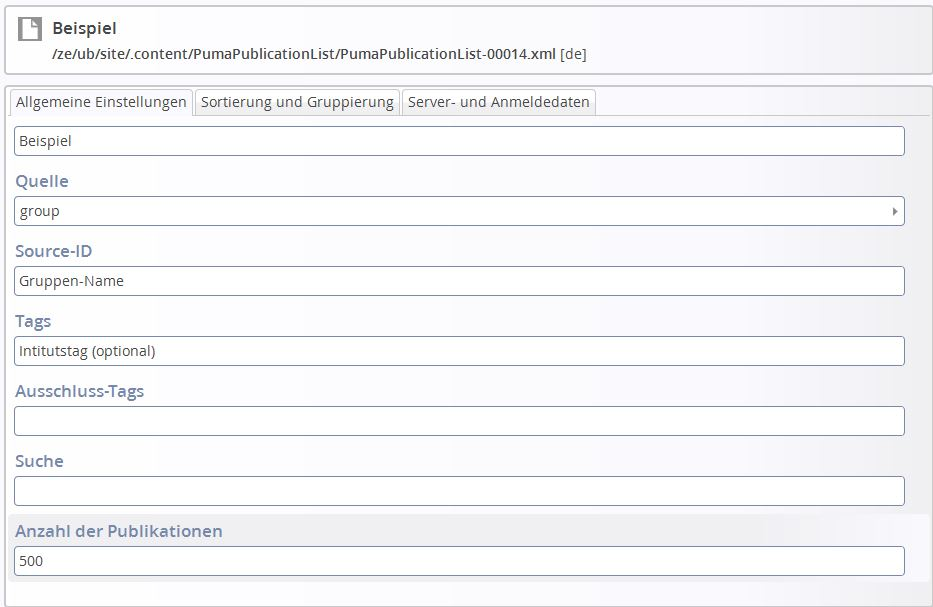
\includegraphics[width=8cm]{Bilder/Kapitel9/Institutsliste1.JPG}
 \caption{Allgemeine Einstellungen}
 \label{fig:iplAllgemeineEinstellungen}
\end{figure}\begin{figure}[h!]
 \centering
 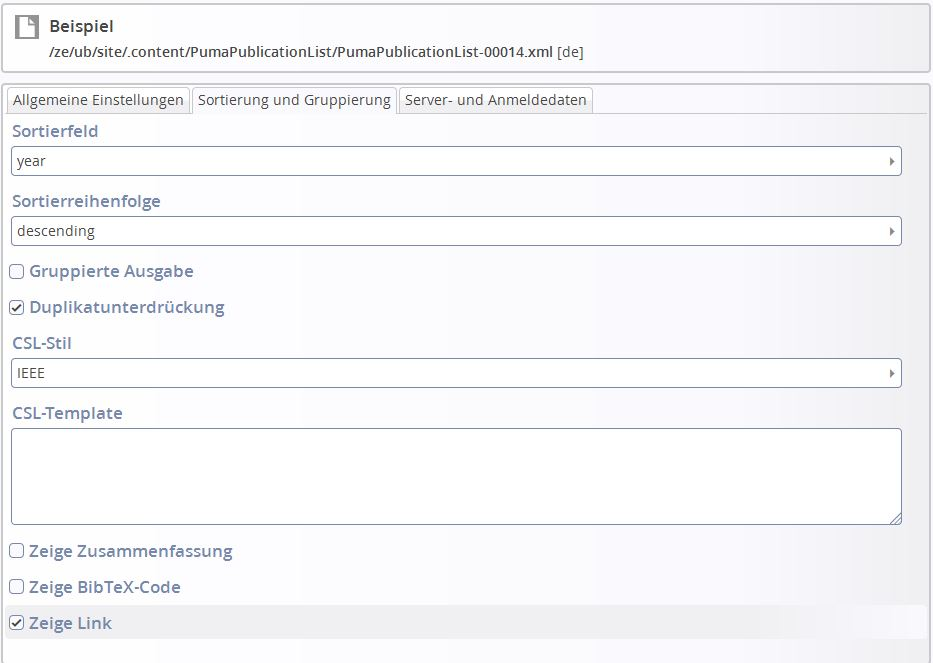
\includegraphics[width=8cm]{Bilder/Kapitel9/Institutsliste2.jpeg}
 \caption{Sortierung und Gruppierung}
 \label{fig:iplSortierungGruppierung}
\end{figure}\begin{figure}[h!]
 \centering
 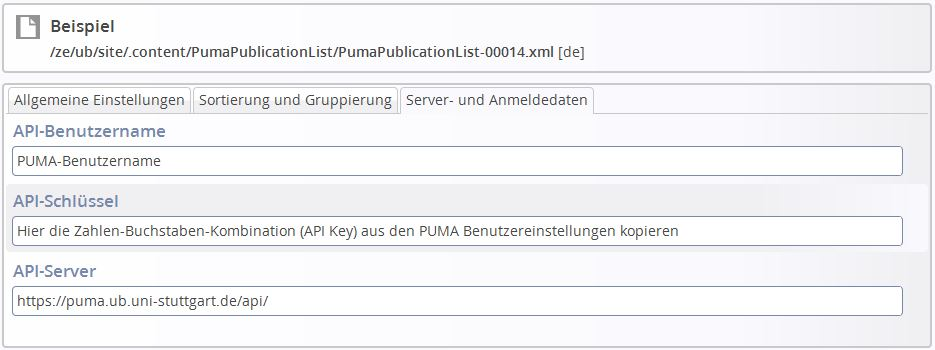
\includegraphics[width=8cm]{Bilder/Kapitel9/Institutsliste3.jpeg}
 \caption{Server- und Anmeldedaten}
 \label{fig:iplServerAnmeldedaten}
\end{figure}
\subsubsection*{Beipiel Mitarbeiterpublikationsliste}\label{sss:mpl}
Im folgenden Beispiel zeigen die Abbildungen \ref{fig:mplAllgemeineEinstellungen}, \ref{fig:mplSortierungGruppierung} und \ref{fig:mplServerAnmeldedaten} die Einstellungen zur Ausgabe einer Mitarbeiterpublikationsliste in OpenCms.

\begin{figure}[h!]
 \centering
 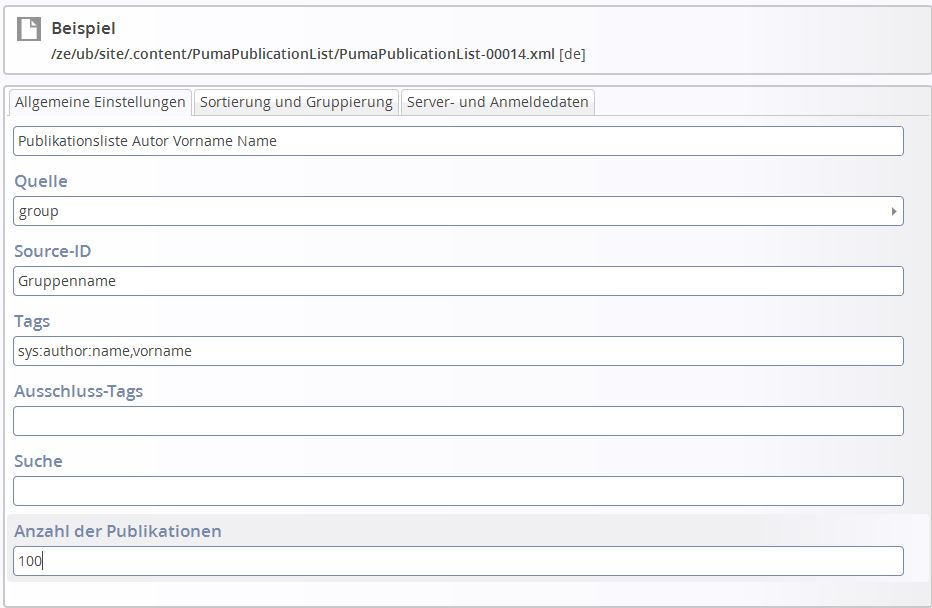
\includegraphics[width=8cm]{Bilder/Kapitel9/Mitarbeiterliste1.jpeg}
 \caption{Allgemeine Einstellungen}
 \label{fig:mplAllgemeineEinstellungen}
\end{figure}
\begin{figure}[h!]
 \centering
 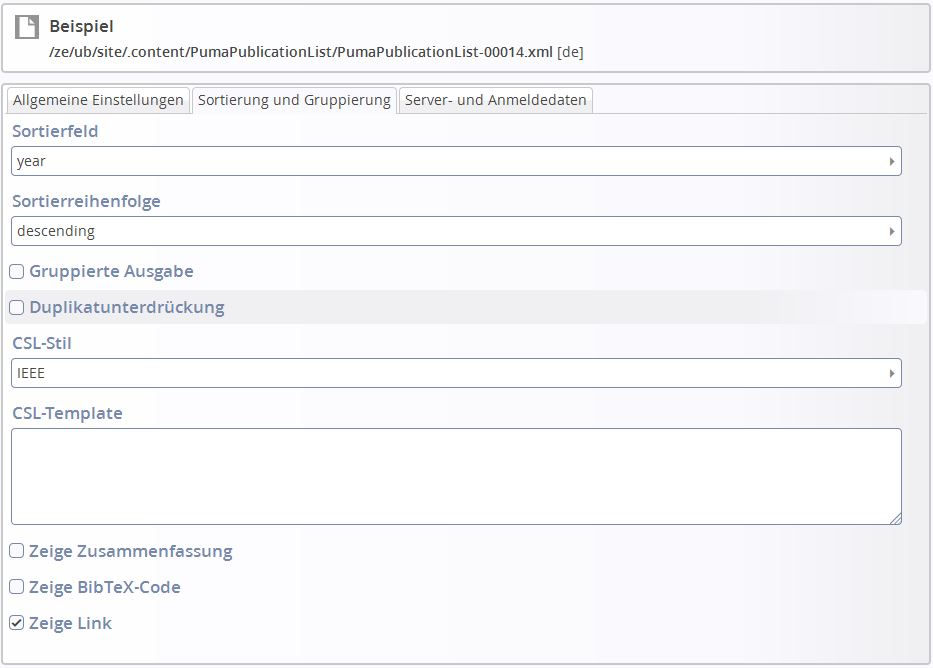
\includegraphics[width=8cm]{Bilder/Kapitel9/Mitarbeiterliste2.jpeg}
 \caption{Sortierung und Gruppierung}
 \label{fig:mplSortierungGruppierung}
\end{figure}
\begin{figure}[h!]
 \centering
 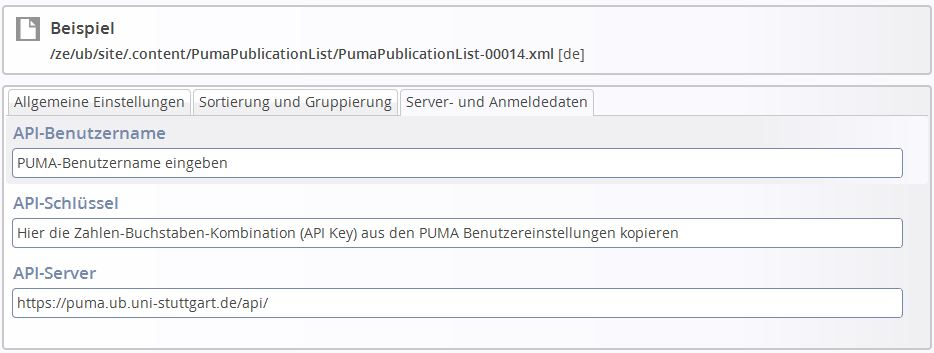
\includegraphics[width=8cm]{Bilder/Kapitel9/Mitarbeiterliste3.jpeg}
 \caption{Server- und Anmeldedaten}
 \label{fig:mplServerAnmeldedaten}
\end{figure}
Wenn die gewünschten Einstellungen veröffentlicht werden, importiert das Plugin die Literatureinträge im ausgewählten Zitationsstil auf die entsprechenden OpenCms-Seite. Veränderungen, die bei PUMA vorgenommen werden, Korrekturen oder weitere Einträge werden automatisch auf der OpenCms-Seite aktualisiert. Durch das Caching in OpenCms können Änderungen im PUMA-System zeitverzögert in OpenCms sichtbar werden.
\subsection{Typo3\index{Typo3}}
\label{subsec:typo3}
\subsubsection*{Installation}\label{sss:installation}
PUMA CSL ist eine Erweiterung (Extension) für Typo3\index{Plugins!Typo3}. Um sie zu installieren, suchen Sie im Extension Manager nach der Extension ext\_bibsonomy\_csl und importieren Sie diese.
\begin{figure}[h!]
 \centering
 \fbox{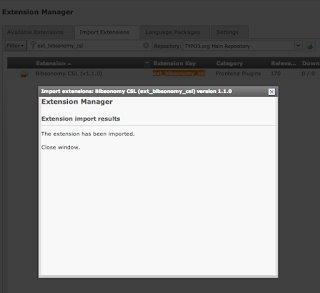
\includegraphics[width=8cm]{Bilder/Kapitel9/extension_manager.jpg}}
 \caption{Extension Manager}
 \label{fig:extensionManager}
\end{figure}
Nach erfolgreichem Import wird die Extension unter \enquote{Available Extensions} angezeigt. Klicken Sie auf das +-Symbol, um es zu aktivieren.
\begin{figure}[h!]
 \centering
 \fbox{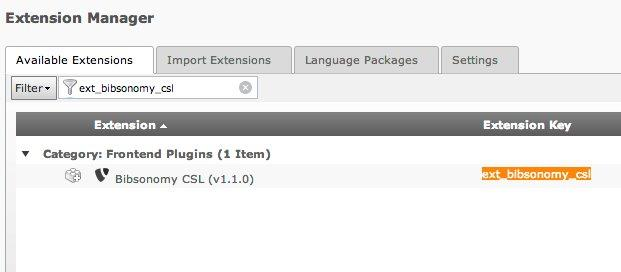
\includegraphics[width=11cm]{Bilder/Kapitel9/available_extensions.jpg}}
 \caption{Available Extensions}
 \label{fig:availableExtensions}
\end{figure}

\subsubsection*{Publikationslisten hinzufügen mit dem Frontend Plugin}\label{sss:typo3Publikationslisten}
Nachdem Sie die Extension importiert und aktiviert haben, können Sie Publikationslisten erstellen. Fügen Sie dazu der Seite, auf der die Publikationsliste erscheinen soll, ein neues Plugin hinzu. Wählen Sie hierfür aus der Liste \enquote{PUMA Publication List} aus.\newline
\newline
Im Reiter \enquote{General} tragen Sie den Titel für die Publikationsliste ein.
\begin{figure}[h!]
 \centering
 \fbox{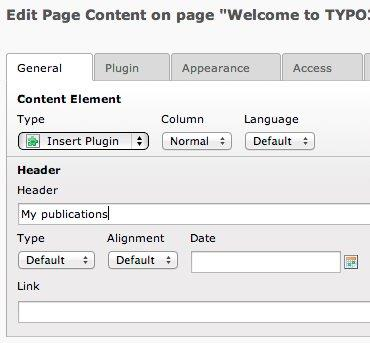
\includegraphics[width=8cm]{Bilder/Kapitel9/reiter_general.jpg}}
 \caption{Reiter General}
 \label{fig:reiterGeneral}
\end{figure}

Gehen Sie auf den Reiter \enquote{Plugin} und nehmen Sie die gewünschten Einstellungen vor. Sie können zwischen den Inhaltstypen \textit{user}, \textit{group} oder \textit{viewable} wählen, um zu definieren, ob die Publikationsliste aus den Einträgen eines Benutzers, einer Gruppe oder einer Sichtbarkeitseinstellung bestehen soll. Geben Sie im untersten Textfeld als \textit{custom url} die Seite Ihrer PUMA-Installation ein, also \textit{http://puma.ub.uni-stuttgart.de}\newline
\newline
Beispiel: Sie möchten Ihre eigene Publikationsliste einbinden. Dazu wählen Sie zunächst unter der Rubrik \enquote{Content Source} die Option \enquote{user} aus. Tragen Sie dann den gewünschten (Ihren) Nutzernamen unter \enquote{Insert the id of user, group or viewable source} ein. Anschließend können Sie die Einträge der Publikationsliste über Tags filtern. Geben Sie hierfür die gewünschten Tags in das Feld \enquote{Select content via tags} ein. Um nur eigene Einträge anzeigen zu lassen, verwenden Sie das Systemtag \textit{myown}. Sie können zudem die Anzahl der angezeigten Publikationen begrenzen sowie mittels Freitext filtern.
\begin{figure}[h!]
 \centering
 \fbox{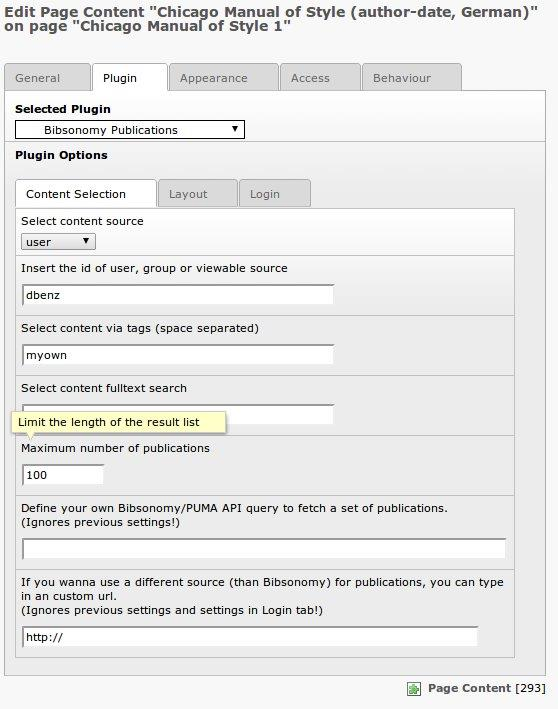
\includegraphics[width=9cm]{Bilder/Kapitel9/reiter_plugin.jpg}}
 \caption{Reiter Plugin}
 \label{fig:reiterPlugin}
\end{figure}

\begin{mdframed}[style=mdfexample1,frametitle={ACHTUNG},backgroundcolor=gray!40]Bitte beachten Sie, dass die Extension Ihre gesamte Publi\-kations\-liste darstellt, wie Sie sie in PUMA sehen \textbf{(auch private Publikationen)}. Wenn Sie z.B. an eine Publikation ein Dokument angehängt haben, dann wird dieses auch in der Publikationsliste angezeigt. Dadurch können für Sie \textbf{urheberrechtliche Konsequenzen} entstehen. Wir empfehlen Ihnen daher für die Nutzung einen zusätzlichen Account anzulegen, mit dem Sie in PUMA nur die TYPO3-Publikationen verwalten.
\end{mdframed} 
Im Reiter \enquote{Layout} können Sie den Zitationsstil der Publikationsliste anpassen. Die Definition des Zitationsstils geschieht mit Hilfe der Citation Style Language (CSL\index{CSL}). Eine große Liste an frei verfügbaren CSL-Vorlagen finden Sie unter: \url{http://www.zotero.org/styles/}.
\begin{figure}[h!]
 \centering
 \fbox{
\includegraphics[width=7cm]{Bilder/Kapitel9/csl_typo.jpg}}
 \caption{Citation Style Language(CSL)}
 \label{fig:csl}
\end{figure}

Im Reiter Rubrik \enquote{Login} müssen Sie Ihre PUMA
API-Daten\index{API} hinterlegen. Nur so kann sich die TYPO3 Extension
bei PUMA anmelden und Ihre Daten abrufen. Ihren API-Key finden Sie,
wenn Sie im Benutzermenü (\autoref{sec:benutzermenue}) in die
Einstellungen gehen und im Reiter \enquote{Einstellungen} nach unten
scrollen.

\subsubsection*{Tag-Wolken hinzufügen mit dem Frontend Plugin}\label{sss:typo3Tagwolken}
Sie können Ihren Typo3-Seiten nicht nur Publikationslisten hinzufügen, sondern auch Ihre PUMA Tag-Wolke (Tagcloud). Fügen Sie dazu der Seite, auf der die Tag-Wolke\index{Tag!Wolke} erscheinen soll, ein neues Plugin hinzu. Wählen Sie aus der Liste \enquote{Bibsonomy Tag Cloud}.

Wie in \autoref{sss:typo3Publikationslisten} können Sie auch hier zwischen verschiedenen Modi wählen.
\subsubsection*{CSL Styles verwalten}\label{typo3CslBackend}

Bei der Installation der Extension werden Ihnen eine Reihe von CSL-Stylesheets ausgeliefert. Um weitere Stylesheets hinzuzufügen, erstellen Sie einen neuen Ordner im Seitenbaum und nennen diesen \textit{CSL Styles}. Wählen Sie anschließend diesen Ordner aus. Klicken Sie auf \enquote{Neu} und wählen \enquote{Add a custom style}.

\autoref{fig:neueStylesheets} zeigt die drei unterschiedlichen Möglichkeiten, ein neues Stylesheet anzulegen:
\begin{enumerate}
\item Geben Sie den CSL-Quellcode direkt in das Textfeld ein und klicken Sie anschließend auf \enquote{Save}.
\item Geben Sie in das Textfeld die URL des CSL-Stylesheets ein und klicken Sie auf \enquote{Import}.
\item Laden Sie ein CSL-Stylesheet von Ihrem Computer hoch, indem Sie auf \enquote{Upload} klicken. 
\end{enumerate}
\begin{figure}[h!]
 \centering
 \fbox{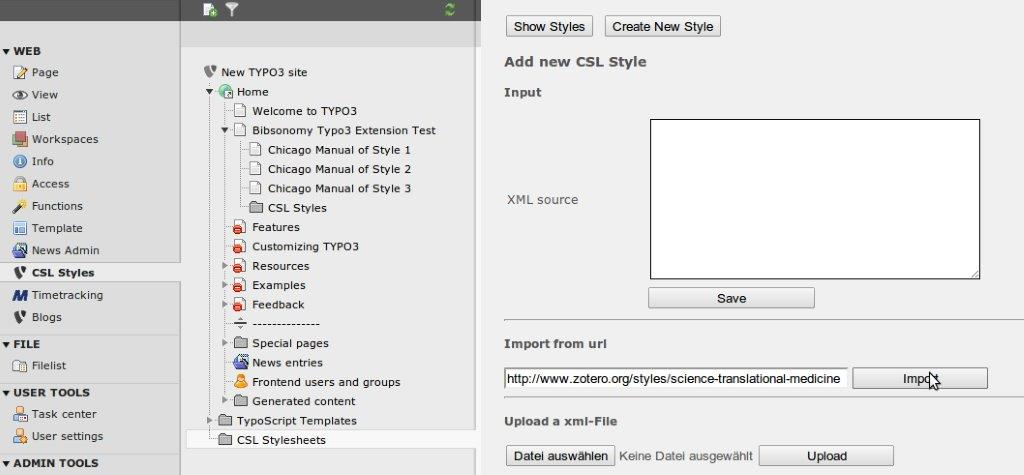
\includegraphics[width=11cm]{Bilder/Kapitel9/stylesheets.jpg}}
 \caption{Neue Stylesheets hinzuzufügen}
 \label{fig:neueStylesheets}
\end{figure}
Um eine Vorschau zu erhalten, klicken Sie auf \enquote{Show Styles}.\newline
Um ein CSL-Stylesheet zu löschen, klicken Sie wie gewohnt auf das Mülleimersymbol in Typo3. 
\begin{figure}[h!]
 \centering
 \fbox{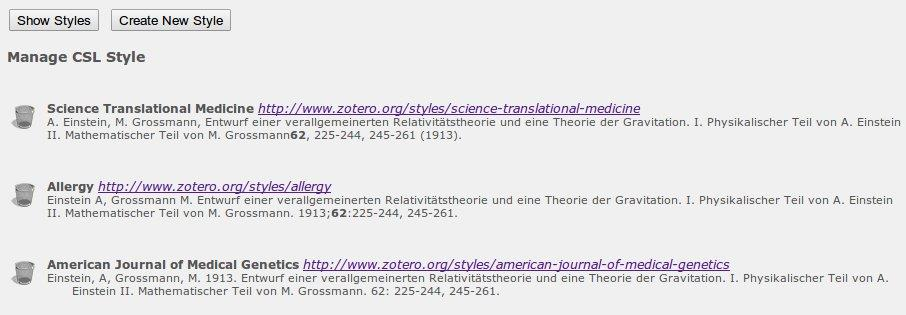
\includegraphics[width=11cm]{Bilder/Kapitel9/csl_stylesheet.jpg}}
 \caption{CSL-Stylesheet löschen}
 \label{fig:cslLoeschen}
\end{figure}
\subsection{WordPress\index{WordPress}}
\label{subsec:wordpress}
Um Publikationslisten aus PUMA in eine WordPress-Seite einzufügen, wird das WordPress-Plugin\index{Plugins!WordPress} \textit{BibSonomy/PUMA CSL} oder das Plugin \textit{BibSonomy/PUMA CSL - Publications \& Tag Cloud Widget}\footnote{\url{https://wordpress.org/plugins/bibsonomy-csl/}} benötigt. Eine ausführliche Anleitung zur Installation und Nutzung finden Sie im BibSonomy Blog. \footnote{\url{http://blog.bibsonomy.org/2012/12/feature-of-week-add-publication-lists.html}} Aktivieren Sie das Plugin und das TagCloudWidget im Plugins-Menü von Wordpress. Beides wurde vom PUMA-Team der UB Stuttgart zuletzt erfolgreich mit der WordPress-Version 4.9.5 getestet.

Nach der Installation finden Sie im Menü \enquote{Einstellungen} einen neuen Eintrag namens \textit{BibSonomy CSL}. Geben Sie dort als BibSonomy Host \textit{puma.ub.uni-stuttgart.de}, als user ID Ihren PUMA-Benutzernamen und als API key ihren individuellen API key ein, den Sie im Benutzermenü in den Einstellungen finden (siehe \autoref{subsec:apiAuth}).  

\subsubsection*{Publikationslisten hinzufügen}
\label{sss:wordpressPublist}

In WordPress finden Sie nun bei Seiten und Beiträgen eine neue Meta-Box namens \textit{Add BibSonomy Publications}, mit der Sie PUMA-Publikationen in die Seite einfügen können. Sie legen die Auswahl der Publikationen mit Hilfe der folgenden Felder fest:

\begin{description}
\item [Inhaltstyp (content type)] \hfill \\
  Hier können Sie wählen, ob Sie die Publikationen eines bestimmten Benutzers (\textit{user}), einer Gruppe (\textit{group}) oder eines Sichtbarkeitstyps (\textit{viewable}) einfügen möchten.
\item [Inhaltstyp-Wert (value of content type)] \hfill \\
  Hier geben Sie den Benutzernamen (bei Inhaltstyp \textit{user}), den Gruppennamen (bei Inhaltstyp \textit{group}) oder den Sichtbarkeitstyp (bei Inhaltstyp \textit{viewable}) an.
\item [Tags] \hfill \\
  Hier können Sie die Ergebnisliste einschränken, indem Sie Tags angeben, mit denen die Publikationen annotiert sein müssen. Mehrere Tags werden durch Leerzeichen getrennt.
\item [Volltext-Suchbegriff (fulltext search)] \hfill \\
  Hiermit können Sie die Ergebnisliste durch einen Suchbegriff einschränken, nachdem die Ergebnisse per Volltextsuche durchsucht werden.
\item [Länge der Ergebnisliste (length of the result list)] \hfill \\
  Hier geben Sie an, wie viele Einträge angezeigt werden sollen.
\item [CSL-Stylesheet] \hfill \\
  Hier wählen Sie den Zitationsstil aus, nach dem die Ergebnisse ausgegeben werden sollen. Ist der gewünschte Stil nicht im Drop-Down-Menü vorhanden, können Sie auch alternativ eine URL angeben.
\item [Show link to abstract] Link zur Zusammenfassung in der Publikationsliste anzeigen lassen.
\item [Show URL, BibTeX and EndNote links] Link zum BibTeX- oder EndNote-Code ausgeben.
\item [Show download links] Links zum Download von Dokumenten, die mit dem Publikationseintrag verknüpft sind.
\item [Show thumbnails of documents] Anzeige von Vorschaubildern zu den Dokumenten. 
\item [Group publications by year] Publikationsliste nach Veröffentlichungsjahr gruppieren (mit Jahreszahl als Zwischenüberschrift), mit und ohne Sprungmarken.
\item [CSS] \hfill \\
  Hier können Sie die Ausgabe der Publikationen mit Hilfe von CSS-Code genauer steuern.
\end{description}

Um zum Beispiel die Liste der eigenen Publikationen anzuzeigen, wählen Sie beim Inhaltstyp \textit{user}, geben als Wert Ihren Benutzernamen und als Tag \textit{myown} an. 


\subsubsection*{Tagwolken hinzufügen}
\label{sss:wordpressTagcloud}

Um in WordPress eine Tagwolke (Tagcloud) einzufügen, aktivieren Sie das TagCloudWidget. Anschließend können Sie auf der Widget-Seite im Design-Menü das BibSonomy/PUMA TagCloud-Widget an die gewünschte Stelle ziehen. Auch hier können Sie beim Inhaltstyp (source type) wählen, ob sich die Tag-Wolke auf die Sammlung von Publikationen eines Benutzers (\textit{user}), einer Gruppe (\textit{group}) oder auf alle öffentlich geteilten Einträge (\textit{viewable}) beziehen soll. Bei \textit{BibSonomy source type value} tragen Sie dann entsprechend entweder Ihren Benutzernamen, den gewünschten Gruppennamen oder \enquote{public} ein. Drei Layouts stehen zur Verfügung: Simple, Decorated, Button Style. Die Überschrift kann auch weggelassen werden. Die angezeigten Tags verlinken auf die dazugehörigen Einträge in PUMA.


\subsection{Zope\index{Zope}}
\label{subsec:zope}
Sie können Inhalte aus PUMA in das Content Management System Zope\footnote{\url{http://www.zope.org/}} integrieren.
\begin{enumerate}
    \item Publikationen\newline
    Publikationslisten können mit Hilfe von \textit{RDF Summary}\footnote{\url{http://old.zope.org/Members/EIONET/RDFSummary/}} als RSS-Feeds\index{RSS} (siehe \autoref{subsec:export}) in Ihre Zope-Seite integriert werden. 
    \item Tagwolken\newline
    Sie haben die Möglichkeit, mit Hilfe von \textit{Kebas Data}\footnote{\url{https://sourceforge.net/projects/kebasdata/}} Tagwolken auf Ihren Zope-Seiten einzufügen. Eine detaillierte Anleitung hierfür findet sich unter \footnote{\url{https://puma.uni-kassel.de/help_de/Tag-Wolken\%20auf\%20Zope-Seiten}}
\end{enumerate}
%\subsubsection*{Tag-Wolken auf Zope-Seiten} \label{sss:zopeTagwolken}
%PUMA-Schlagwörter können auf einer Zope-Seite angezeigt werden. 
%\begin{enumerate}
%    \item Sie müssen auf eine PUMA-Seite aus Zope heraus zugreifen. Hierfür benötigen Sie das Produkt Kebas Data .
%    \item Für jede Tag-Wolke, die Sie anzeigen lassen wollen, benötigen Sie ein KebasData-Objekt. Bitte konfigurieren Sie es wie folgt (Benutzername etc. muss entsprechend ersetzt werden):
%  
%\begin{figure}[h!]
% \centering
% 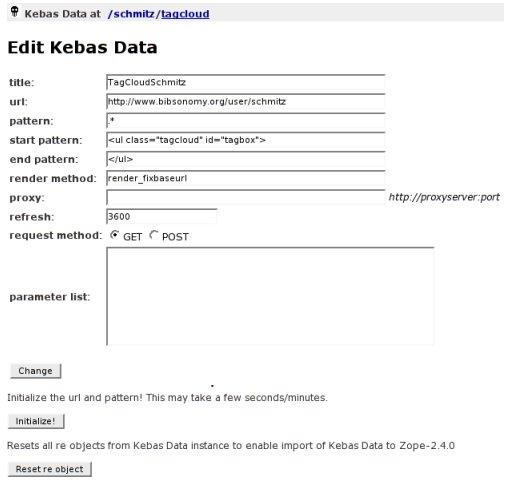
\includegraphics[width=11cm]{Bilder/tag_wolken.jpg}
% \caption{KebayData-Objekt für Tag-Wolken}
% \label{fig:kebayDataObjekt}
%\end{figure}
%
%    Es werden nun alle Tags in Ihrer Tag-Wolke angezeigt, die sich zwischen den Start- <ul ...> und den Ende- </ul> Schemata bewegen.
%    \item Sie müssen jedoch die von PUMA ausgegebenen URLs überarbeiten, da diese sich auf das PUMA-Hauptverzeichnis und nicht auf Ihre Seite beziehen. Hierfür fügen Sie bitte ein \enquote{Script (Python)}-Objekt namens \textit{render\_fixbaseurl} in Zope an beliebiger Stelle oberhalb des Ordners ein, der Ihre Tag-Wolke enthält. Lassen Sie es zwei Parameter haben und folgendermaßen aussehen: 
%
%    ul = context.match[0]\newline
%    ul = ul.replace('href="/', 'href="https://puma.ub.uni-stuttgart.de/')\newline
%    print ul\newline
%    return printed\newline
%    some code block
%
%    \item Für die Anzeige Ihrer Tag-Wolke von \textit{DTML} aus müssen Sie diesen Befehl eingeben: 
%
%    <ul class="tagbox">\newline
%        <dtml-var tagcloud>\newline
%    </ul> \newline
%
%    \item Für die Anzeige Ihrer Tag-Wolke von einem \textit{Page Template} aus können Sie diesen Befehl benutzen: 
%
%    <ul class=\"tagbox\">\newline
%        <div tal:replace="structure here/tagcloud"/>\newline
%    </ul>\newline
%
%    \item Nutzen Sie CSS\index{CSS} zur Formatierung der Tag-Wolke nach Ihrem Geschmack. Hier sehen Sie, was wir benutzen; bitte beachten Sie, dass dies die selten vorkommenden Tags verbirgt. Sie können \textit{display: none} durch \textit{display: inline} ersetzen, um deren Anzeige zu aktivieren: 
%
%    ul.tagbox \{ list-style: none; text-align: justify; \}\newline
%    ul.tagbox li \{ display: inline; \}\newline
%    ul.tagbox li a \{ display: none; text-decoration: none; color: \#e05698; font-size: 60\% \} \newline
%    ul.tagbox li.tagone a \{  display: none; text-decoration: none; color: \#a3004e; font-size: 80\% \} \newline
%    ul.tagbox li.tagten a \{  display: inline; text-decoration: none; color: \#830030; font-size: 100\% \} \newline
%\end{enumerate}
%


%\subsection{Ilias}
%\label{subsec:ilias}
%\subsection{Moodle}
%\label{subsec:moodle}
%https://moodle.org/plugins/pluginversion.php?id=12514
%Das PUMA/BibSonomy Module (PBM) ist das PUMA/BibSonomy Plugin für Moodle. Es ermöglicht das Veröffentlichen von Publikationslisten aus PUMA heraus in einen Moodlekurs. Der Zitationsstil, in welchem die Publikationen in Moodle angezeigt werden sollen, kann mit Hilfe des CSL\footnote{\url{http://citationstyles.org/}} festgelegt werden.\newline\newline
%\textbf{ Der Administrator}\newline
%Die folgenden Schritte sind wichtig für die Installation des PBM Plugins: 
%\begin{enumerate}
	%\item Laden Sie sich das Plugin als \*.zip Datei herunter. Wählen Sie auf der Seite von Moodle (\url{https://moodle.org/plugins/view.php?plugin=mod_pbm} ) den Reiter \enquote{Version} aus und klicken auf Download.
	%\item Entpacken Sie die \*.zip Datei im  richtigen Ordner (z.B. /var/www/moodle/mod/pbm)
	%\item Gehen Sie auf die Moodle Webseite und loggen Sie sich als Administrator ein. Gehen Sie unter Einstellungen auf \enquote{Website-Administration} wählen Sie \enquote{Plugins} aus. Klicken Sie anschließend auf\enquote{Plugin-Übersicht}.
	%\item Klicken Sie oben auf der Überblickseite der Plugins auf den Button \enquote{Alle verfügbaren Updates überprüfen}.
	%\item Moodle informiert Sie darüber, dass das Database Update durchgeführt wurde. Bestätigen Sie dies.     
	%\item Sie werden nach einer voreingestellten Serveradresse gefragt, nach Ihren OAuth Consumer-Daten und Ihrer Wahl des Zitationsstils.      
%\end{enumerate}   
%Für die Konfiguration füllen Sie bitte folgende Felder aus:\newline\newline   
%\textbf{Default PBM Server:} Fügen Sie in dieses Feld die URL von PUMA Stuttgart ein (\url{https://puma.ub.uni-stuttgart.de/}). Diese wird ab sofort als Standard verwendet, wenn ein PBM zum Moodle-Kurs hinzugefügt wird.\newline\newline
%\textbf{Comsumer-Key/Consumer-Secret(Optional):}Der Administrator eines Moodle-Kurses kann in den lokalen Administrations-Einstellungen eine OAuth -Nutzer- Bestätigung erstellen. Diese wird dazu verwendet, um die Accounts der Nutzer über die OAuth Authentifizierung mit PUMA zu verknüpfen. \newline\newline
%\textbf{Available CSL files:}Hier können Sie zwischen unterschiedlichen Zitationsstilen auswählen. Weitere Informationen über Zitationsstile gibt es unter \url{http://citationstyles.org/}.
%\newline\newline
%\textbf{Nutzer}\newline
\section{Probleme melden}
\label{sec:bitbucket}
Die Weiterentwicklung von PUMA wird über Bitbucket\index{Bitbucket} verwaltet. Bitbucket ist ein auf Git basierendes Versionskontrollsystem, das die Zusammenarbeit innerhalb von Entwicklungs-Teams erleichtert.  

Fehler innerhalb von PUMA können in Bitbucket an die Entwickler gemeldet werden. Hierzu benötigt man ein eigens Bitbucket-Nutzerkonto. Mit diesem melden Sie sich bei Bitbucket an und gehen auf die Bibsonomy/~Puma-Seite\footnote{\url{https://bitbucket.org/bibsonomy/puma}}. Unter dem Reiter \enquote{Issues} können neue Problemmeldungen verfasst werden.
